\documentclass[journal,12pt,twocolumn]{IEEEtran}
%
\usepackage{setspace}
\usepackage{gensymb}
%\doublespacing
\singlespacing

\usepackage{graphicx}
\usepackage[cmex10]{amsmath}
\usepackage{amsmath,amsthm}
\usepackage{mathrsfs}
\usepackage{txfonts}
\usepackage{stfloats}
\usepackage{bm}
\usepackage{cite}
\usepackage{cases}
\usepackage{subfig}

\usepackage{longtable}
\usepackage{multirow}
\usepackage{commath}
\usepackage{enumitem}
\usepackage{mathtools}
\usepackage{steinmetz}
\usepackage{tikz}
\usepackage{circuitikz}
\usepackage{verbatim}
\usepackage{tfrupee}
\usepackage[breaklinks=true]{hyperref}

\usepackage{tkz-euclide}

\usetikzlibrary{calc,math}
\usepackage{listings}
\usepackage{color}                                            
\usepackage{array}                                            
\usepackage{longtable}                                        
\usepackage{calc}                                             
\usepackage{multirow}                                         
\usepackage{hhline}                                           
\usepackage{ifthen}                                           
\usepackage{lscape}     
\usepackage{multicol}
\usepackage{chngcntr}

\DeclareMathOperator*{\Res}{Res}

\renewcommand\thesection{\arabic{section}}
\renewcommand\thesubsection{\thesection.\arabic{subsection}}
\renewcommand\thesubsubsection{\thesubsection.\arabic{subsubsection}}

\renewcommand\thesectiondis{\arabic{section}}
\renewcommand\thesubsectiondis{\thesectiondis.\arabic{subsection}}
\renewcommand\thesubsubsectiondis{\thesubsectiondis.\arabic{subsubsection}}

\hyphenation{op-tical net-works semi-conduc-tor}
\def\inputGnumericTable{}                                 

\lstset{
	%language=C,
	frame=single, 
	breaklines=true,
	columns=fullflexible
}
\lstset{
	%language=TeX,
	frame=single, 
	breaklines=true
}

\begin{document}
	
	
	\newtheorem{theorem}{Theorem}[section]
	\newtheorem{problem}{Problem}
	\newtheorem{proposition}{Proposition}[section]
	\newtheorem{lemma}{Lemma}[section]
	\newtheorem{corollary}[theorem]{Corollary}
	\newtheorem{example}{Example}[section]
	\newtheorem{definition}[problem]{Definition}
	
	\newcommand{\BEQA}{\begin{eqnarray}}
		\newcommand{\EEQA}{\end{eqnarray}}
	\newcommand{\define}{\stackrel{\triangle}{=}}
	\bibliographystyle{IEEEtran}
	\providecommand{\mbf}{\mathbf}
	\providecommand{\pr}[1]{\ensuremath{\Pr\left(#1\right)}}
	\providecommand{\qfunc}[1]{\ensuremath{Q\left(#1\right)}}
	\providecommand{\sbrak}[1]{\ensuremath{{}\left[#1\right]}}
	\providecommand{\lsbrak}[1]{\ensuremath{{}\left[#1\right.}}
	\providecommand{\rsbrak}[1]{\ensuremath{{}\left.#1\right]}}
	\providecommand{\brak}[1]{\ensuremath{\left(#1\right)}}
	\providecommand{\lbrak}[1]{\ensuremath{\left(#1\right.}}
	\providecommand{\rbrak}[1]{\ensuremath{\left.#1\right)}}
	\providecommand{\cbrak}[1]{\ensuremath{\left\{#1\right\}}}
	\providecommand{\lcbrak}[1]{\ensuremath{\left\{#1\right.}}
	\providecommand{\rcbrak}[1]{\ensuremath{\left.#1\right\}}}
	\theoremstyle{remark}
	\newtheorem{rem}{Remark}
	\newcommand{\sgn}{\mathop{\mathrm{sgn}}}
	\providecommand{\abs}[1]{\(\left\vert#1\right\vert\)}
	\providecommand{\res}[1]{\Res\displaylimits_{#1}} 
	\providecommand{\norm}[1]{\(\left\lVert#1\right\rVert\)}
	%\providecommand{\norm}[1]{\lVert#1\rVert}
	\providecommand{\mtx}[1]{\mathbf{#1}}
	\providecommand{\mean}[1]{E\(\left[ #1 \right]\)}
	\providecommand{\fourier}{\overset{\mathcal{F}}{ \rightleftharpoons}}
	%\providecommand{\hilbert}{\overset{\mathcal{H}}{ \rightleftharpoons}}
	\providecommand{\system}{\overset{\mathcal{H}}{ \longleftrightarrow}}
	%\newcommand{\solution}[2]{\textbf{Solution:}{#1}}
	\newcommand{\solution}{\noindent \textbf{Solution: }}
	\newcommand{\cosec}{\,\text{cosec}\,}
	\providecommand{\dec}[2]{\ensuremath{\overset{#1}{\underset{#2}{\gtrless}}}}
	\newcommand{\myvec}[1]{\ensuremath{\begin{psmallmatrix}#1\end{psmallmatrix}}}
	\newcommand{\mydet}[1]{\ensuremath{\begin{vmatrix}#1\end{vmatrix}}}
	%\numberwithin{equation}{section}
	\numberwithin{equation}{subsection}
	%\numberwithin{problem}{section}
	%\numberwithin{definition}{section}
	\makeatletter
	\@addtoreset{figure}{problem}
	\makeatother
	\let\StandardTheFigure\thefigure
	\let\vec\mathbf
	%\renewcommand{\thefigure}{\theproblem.\arabic{figure}}
	\renewcommand{\thefigure}{\theproblem}
	%\setlist[enumerate,1]{before=\renewcommand\theequation{\theenumi.\arabic{equation}}
	%\counterwithin{equation}{enumi}
	%\renewcommand{\theequation}{\arabic{subsection}.\arabic{equation}}
	\def\putbox#1#2#3{\makebox[0in][l]{\makebox[#1][l]{}\raisebox{\baselineskip}[0in][0in]{\raisebox{#2}[0in][0in]{#3}}}}
	\def\rightbox#1{\makebox[0in][r]{#1}}
	\def\centbox#1{\makebox[0in]{#1}}
	\def\topbox#1{\raisebox{-\baselineskip}[0in][0in]{#1}}
	\def\midbox#1{\raisebox{-0.5\baselineskip}[0in][0in]{#1}}
	\vspace{3cm}
	\title{Assignment 7}
	\author{Addagalla Satyanarayana}
	\maketitle
	\newpage
	%\tableofcontents
	\bigskip
	\renewcommand{\thefigure}{\theenumi}
	\renewcommand{\thetable}{\theenumi}
\begin{abstract}
This document uses the properties of a parabola
\end{abstract}
Download latex-tikz codes from 
%
\begin{lstlisting}
https://github.com/AddagallaSatyanarayana/AI5106/tree/master/Assignment7/Assignment7.tex
\end{lstlisting}
%
\section{Problem}
	Trace the parabola
\begin{align}
	144x^2-120xy+25y^2+619x-272y+663=0\label{eq:1}
\end{align}

\section{Explanation}
The general equation of second degree is given by
\begin{align}
	ax^2+2bxy+cy^2+2dx+2ey+f=0 \label{gen_quad_eqn}
\end{align}
and can be expressed as
\begin{align}
	\vec{x}^T\vec{V}\vec{x}+2\vec{u}^T\vec{x}+f=0 \label{conic_quad_eqn}
\end{align}
where
\begin{align}
	\vec{V} &= \vec{V}^T = \myvec{a & b \\ b & c}
	\\
	\vec{u}^T &= \myvec{d & e}
\end{align}

From equation \eqref{eq:1} , we get

\begin{align}
	\vec{V} &= \myvec{144&-60\\-60&25}\label{eq:2}\\
	\vec{u} &= \myvec{\frac{619}{2}\\-\frac{272}{2}}\label{eq:3}\\ 
	f &= 663 \label{eq:conics/ex/solution/given2}
\end{align}
Expanding the determinant of $\vec{V}$ we observe, 
\begin{align}
	\mydet{144&-60\\-60&25} = 0 \label{eq:4}
\end{align}
The characteristic equation of $\vec{V}$ is given as follows,
\begin{align}
		\mydet{\lambda\vec{I}-\vec{V}} = \mydet{\lambda-144&60\\60&\lambda-25} &= 0\\
		\implies \lambda^2-169\lambda &= 0\label{eq:5}
\end{align}
 the eigenvalues are given by
\begin{align}
		\lambda_1=0, \lambda_2=169\label{eq:6}    
\end{align}
For $\lambda_1 = 0$, the eigen vector $\vec{p}$ is given by 
\begin{align}
		\vec{V}\vec{p} = 0
\end{align}
Row reducing $\vec{V}$ 
\begin{align}
		\implies
		\myvec{-144&60\\60&-25}\xleftrightarrow[R_2=R_2+5R_1]{R_1=\frac{R_1}{12}}\myvec{-12&5\\0&0}\\
		\implies\vec{p}_1=\frac{1}{13}\myvec{5\\12} \label{eq:7}
\end{align}
Similarly, 
\begin{align}
		\vec{p}_2=\frac{1}{13}\myvec{12\\-5} \label{eq:8}
\end{align}
	Thus,
\begin{align}
		\vec{P}&=\myvec{\vec{p_1}&\vec{p_2}}=\frac{1}{13}\myvec{5&12\\ 12 &-5} 
\end{align}
and its equation is
\begin{align}
		\vec{y^T}\vec{D}\vec{y}&=-2\eta\myvec{1&0}\vec{y}
\end{align}
where
\begin{align}
		\eta=\vec{u}^T\vec{p_1}=-6.5
\end{align}
The focal length of the parabola is given by 
\begin{align}
	\frac{\abs{2\vec{u}^T\vec{p_1}}}{\lambda_2}	= \frac{1}{13}
\end{align}
\begin{align}
		\myvec{\vec{u^T}+\eta\vec{p_1^T} \\ \vec{V}}\vec{c}=
		\myvec{-f \\ \eta\vec{p_1}-\vec{u}} \label{eq:8}
\end{align}
using equations \eqref{eq:2},\eqref{eq:3} and \eqref{eq:8}
\begin{align}
	\myvec{307& -142 \\ 144 & -60 \\  -60 & 25 }\vec{c}=\myvec{-663 \\ -312\\ 130} 
\end{align}
Forming the augmented matrix and row reducing it:
\begin{align}
		\myvec{307 & -142 & -663\\144 & -60 & -312 \\-60 & 25 &130 }\\
		\xleftrightarrow[]{R_3\leftarrow R_3+(5/12)R_2} 
		\myvec{307 & -142 & -663\\144 & -60 & -312 \\0 & 0 &0 }\\
		\xleftrightarrow[]{R_2\leftarrow R_2/12} 
		\myvec{307 & -142 & -663\\12 & -5 & -26 \\0 & 0 &0 }\\
		\xleftrightarrow[]{R_1\leftarrow R_1/(307)} 
		\myvec{1 & -142/307 & -663/307\\12 & -5 & -26 \\0 & 0 &0 }\\
		\xleftrightarrow[]{R_2\leftarrow R_2-12R_1}
		\myvec{1 & -142/307 & -663/307\\0 & 169/307 & -26/307 \\0 & 0 &0}\\ 
		\xleftrightarrow[]{R_2\leftarrow R_2 (307/169)}
		\myvec{1 & -142/307 & -663/307\\0 & 1 & -2/13 \\0 & 0 &0}\\
		\xleftrightarrow[]{R_1\leftarrow R_1 +(142/307)R_2}
		\myvec{1 & 0 & -8903/3991\\0 & 1 & -2/13 \\0 & 0 &0}
\end{align}
Thus the vertex $\vec{c}$ is:
\begin{align}
	\vec{c}=\myvec{ -2.23\\-0.153} 
\end{align}
\begin{figure}[!htbp]
	\centering
	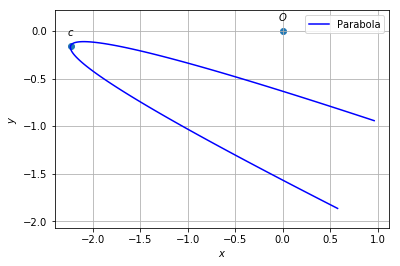
\includegraphics[width =\columnwidth]{parabola.png}
	\caption{Parabola }
	\label{fig:1}
\end{figure}	
\end{document}